
\section{Incomplete Singular Value Decomposition}  \label{sec:isvd}
While SVD is useful for a deeper understanding of the parent matrix, it still does not reduce the number of values needed to represent the parent matrix. In fact, as one can see from \autoref{fig:svdA} the SVD matrices will actually require more values than the parent matrix. However, if we order the singular values and vectors such that $\mtrSig_{11} \ge  \mtrSig_{22} \ge \dots \ge \mtrSig_{mm}$, then for some $k<m$ we can make the approximation:
 \begin{align*}
     \mtrA\mvec{x} &= c_1\mtrSig_{11}\mvec{U}_1 +  c_2\mtrSig_{22}\mvec{U}_2 + \dots + c_n\mtrSig_{mm}\mvec{U}_m \\
     &\approx c_1\mtrSig_{11}\mvec{U}_1 +  c_2\mtrSig_{22}\mvec{U}_2 + \dots + c_n\mtrSig_{kk}\mvec{U}_k \tag{where $k < m$} 
 \end{align*}
This is to say that we are cutting off the action of matrix $\mtrA$ a little early, but, because of the ordering, we are losing as little information as possible. This is called the Incomplete Singular Value Decomposition (ISVD), where we preserve essence of the completed SVD, but it assumes the large  elements of $\mtrSig$ and the corresponding columns in $\mtrU$ and $\mtrV$ matter most, throwing away the columns that are less useful. This will thus allow us to reduce the values need to represent $\mtrA$. This is shown pictorially in \autoref{fig:isvdA}.
\begin{figure}[H]
    \centering
    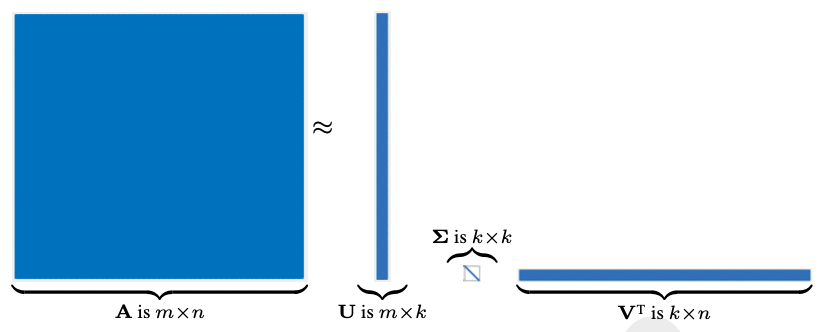
\includegraphics[width=0.6\textwidth]{./imgs/ISVD.jpg}
    \caption{ISVD Representation of $\mtrA$}
    \label{fig:isvdA}
\end{figure}